% a_zer_rename_committer.tex
\documentclass[conference]{IEEEtran}
%\usepackage{babel}
\usepackage{graphicx}
\usepackage{color}
\usepackage{cite}
%\usepackage{algorithmic}
%\usepackage{algorithmicx}
\usepackage[ruled,vlined]{algorithm2e}
\usepackage{listings}
%\usepackage{minted}
\usepackage{underscore}
\usepackage{multicol}
\usepackage{float}

% ========================================================================

\title{
A Zero-rename committer:\\
object-storage as a destination for Apache Hadoop and Spark}

% Yes, this titling is broken
\author{
  Loughran, Steve
  \texttt{stevel@hortonworks.com}\\
\and
  Blue, Ryan
  \texttt{rblue@netflix.com}\\
\and
  Radia, Sanjay
  \texttt{sanjay@hortonworks.com} \\
\and
  Balamohan, Rajesh
  \texttt{rbalamohan@hortonworks.com} \\
}

\date{December 2017}

% ========================================================================

\begin{document}


\maketitle

% ========================================================================

\begin{abstract}

We introduce new \emph{committers} for Apache Hadoop, so permitting
the Amazon S3 Object Store to be used as a direct destination of output generated
by Hadoop MapReduce and Apache Spark.

By using the operations directly exported by
the store, most critically the multipart upload mechanism, these committers upload
their output to the final destination, yet do not materialize this data until the
overall job is committed.
As a result, the committers meet the core requirement of the Hadoop and Spark commit
protocols: output is not visible until committed, while being highly-performant.

We also define the commit protocols of Hadoop and Spark, and show how the classic committer
implementation's requirements of atomic file creation and rename operations mean that they
cannot be safely used with Amazon S3.
hus the new committers are not just ``better'' committers for object stores,
but fundamentally safe for use.

We discuss the two committers, ``Staging'' and ``Magic'', exploring their differences.
The Staging committer stages all generated output to the local filesystem of
worker nodes, uploading this data when a task is committed.
The Magic committer streams data directly to the object store, relying on the
object store client to recognise some output paths as special (``magic''), and
so translating writes to these paths as initiating a delayed-completion write
to a calculated final destination.

\end{abstract}

% ========================================================================

\section{Introduction}
\label{sec:introduction}

It has long been a core requirement of ``Big Data'' computation platforms that
the source and destination of data was a fully consistent distributed filesystem,
albeit often ``sub-POSIX''.

Distributed, because data needs to be readable and writeable by all processes
executing a query across the cluster of computers.
``Sub-POSIX'', in that the full semantics of the POSIX filesystem APIs were not always necessary.
A commonly dropped requirement is the ability to seek past the end of the file and
write data, with a secondary dropped behavior one of being able to overwrite existing
data within a file.
That is: new data could only be written at the current end of the file.
What has been a consistent part of the required semantics has been that the filesystem
presents a model of directories and files with consistent operations to list and
read those directories, and at least four atomic operations:

\begin{itemize}
  \item rename of a single file to another location within the same volume 
  \item rename of a directory and its contents to another location within the same volume 
  \item create file with no overwrite 
  \item recursive delete of a directory 
\end{itemize}

These operations are often used as the foundational operators of higher-level
co-ordination and commit protocols.

For example, the \texttt{create()} operation can be used to obtain a lock on a resource:
the first process to create a file can consider itself having exclusive access to it,
and so implicitly consider itself to have acquired the resource.

The \texttt{rename()} operation is generally critical to providing atomic promotion
of output: a single \texttt{rename()} call can promote all in-progress output
of a worker to become completed work, simply by moving all the output to a well known path.
And, when the job completes, its final output may be renamed to a new location to become
publicly visible.

As covered in\ \cite{MapReduce}:

\begin{quote}
We rely on the atomic rename operation provided by the underlying file system
to guarantee that the final file system state contains just the data produced
by one execution of the reduce task.
\end{quote}


Apache Hadoop was written with its own filesystem, Hadoop Distributed File System (HDFS).

It is self-admittedly ``sub-POSIX'', specifically, while presenting the POSIX
model of a filesystem tree containing directories and files, data can only be
appended directly to the end of the current file.
That is: one my not \texttt{seek()} to before or after the end of the file and
then write data.

It does offer atomic operations which are used in commit protocols and other
applications as a means of enforcing exclusivity;
so permitting the filesystem to act as a mechanism of co-ordinating access across machines.

% ========================================================================

\section{The Hadoop MapReduce Commit Algorithm}
\label{sec:commit}


\subsubsection{Terminology}

First, some terminology needs to be introduced to describe
the protocols.
While much of this terminology is derived from Hadoop's architecture,
some of th e


\textbf{Job}.
A parallelized query/operation to execute.

The output of a Job is made visible to other stages in a larger operation
sequence or other applications if the job \emph{completes successfully}.

\textbf{Job Attempt}.
A single attempt at executing the job;
each one executed from a new set of processes.
Hadoop Jobs are restartable, so more than one attempt may be made;

\textbf{Task}.
A single operation within a job, on a single process, one which generates
one or more files.
A task completes successfully if it generates all the output it expects to without
failing in some way.

\textbf{Task Attempt}.
A single attempt to execute a task.
Multiple attempts may be made to execute a task;
possibly in parallel.
It is critical that only one task attempt's output is propagated
to the final output of a job.


\textbf{Job Driver}.
Whatever process schedules
task execution, tracks success/failures and, determines when all the work has been
processed and then commits the output.
It may also determine that a job
has failed and cannot be recovered, in which case the job is aborted.
In MR and Tez, this is inside the YARN application master.
In Spark it is the driver, which can run in the AM, the YARN client, or other
places (e.g Livy?).


\textbf{Executor}.
A process capable of executing work, as directed by the Job Driver.
In Hadoop, a unique

\textbf{Final directory}.
The directory into which the output of a job is placed
so as to be visible.
After a successful job completion, the data MUST be visible in the final directory.


\textbf{Job Context}.
An instance of the class \texttt{org.apache.hadoop.mapreduce.JobContext},
which provides a read-only view of the Job for the Job Driver and tasks.

\textbf{Task Attempt Context}.
an instance of the class
\texttt{org.apache.hadoop.mapreduce.TaskAttemptContext},
which provides operations for tasks, such as getting and setting status,
progress and counter values.

\textbf{Task Working Directory}.
A directory for exclusive access by a single task,
into which uncommitted work may be placed.

\textbf{Task Commit}.
The act of taking the output of a task attempt and promoting it
to become part of the final output of the active job
attempt.

\textbf{Job Commit}.
The act of taking the output of all committed tasks of a job attempt,
and generating the final output.
This normally consists of publishing this output in an aggregate form;
it can also include generating extra summary data.
As this it is often a serialized operation at the end of a job attempt,
its performance can be a bottleneck.

\textbf{Task Abort}.
To cancel a task such that its data is not committed.

\textbf{Job Abort}.
To cancel all work in a job attempt: no task's work is committed.


\subsection{Requirements of a Commitment Protocol}
\label{subsec:requirementsOfACommitmentProtocol}

Apache Hadoop's MapReduce implementation is designed to support long-lived
large-scale queries taking minutes to hours to complete.
Its requirements include the following:

\begin{enumerate}

  \item Support thousands to tens of thousands of invidually scheduled $tasks$
  within a single $job$.

  \item Support different destinations of work, such as filesystems and databases.

  \item Recover from the failure of a task attempt by rescheduling the task;
  a new task attempt may be executed anywhere within the cluster.

  \item Support speculative execution of task attempts as a means of compensating for the
  delay caused by \emph{stragglers} in the execution.

  \item Potentially: recover from a failure of a job attempt, using all the committed
  task output from the previous, failed attempt.

  \item Be resilient to network failures/partitions of tasks, and of the job manager
  itself becoming isolated from other parts of the system (and hence: a second
  attempt at the job being started).

\end{enumerate}

This leads to some specific requirements of the implementation, requirements
which can be used to assess the correctness of the implementation.

\textbf{Independent.}
Individual tasks must be able to write their data without directly
co-ordinating that write with those of other tasks.

\textbf{Speculative tasks until committed.}
Multiple tasks must be able to simultaneously execute on the same input
source, to generate the required output of that part of the input.
This is required for recovery, and for speculation.
Non requirement: idempotent output;
that is left to the implementors of the operations executed in the tasks.

\textbf{Scaleable communication protocol.}
The commit protocol communications between task and job manager
must be efficient enough to support tens of thousands of simultaneous
tasks.

\textbf{Abortable.}
It must be possible to abort an uncommitted task or job.
There should be no leftover output.

\textbf{Recoverable or Restartable Job.}
A committer can declare whether or not it supports job recovery;
if it does, it must implement recovery.
If not, the job must be restartable from the beginning.

\begin{figure*}
  \centering
  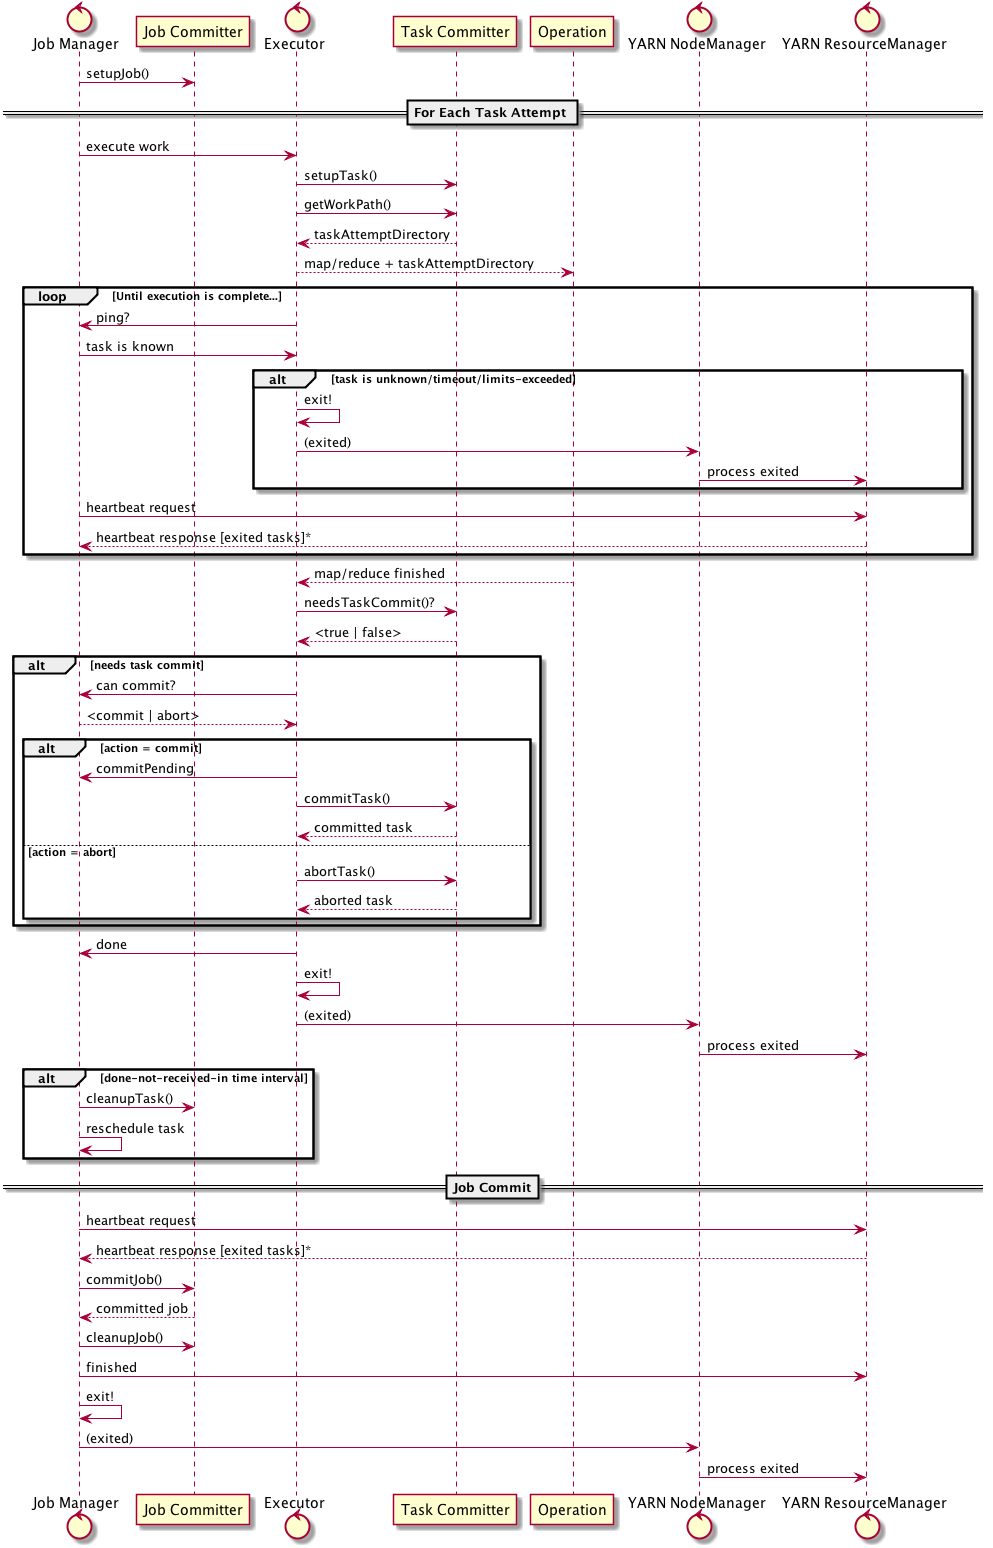
\includegraphics[width=.8\textwidth]{commit-protocol.png}
  \caption{Hadoop commit protocol (excluding Job recovery)}
  \label{fig:commit-protocol}
\end{figure*}

An UML sequence diagram of the core commit protocol is
show in \ref{fig:commit-protocol}.

The commit algorithm is designed to work on the YARN cluster scheduler
\ \cite{Vavilapalli2013}.
This launches the initial Application Master, containing what we call
the ``Job Driver'', and any processes requested by the Application Master
(``the AM'').
On each node in the YARN cluster, a \emph{NodeManager} has the responsibility
of launching the applications, usually within a memory-and-CPU-bounded
environment.
When a launch process terminates, this fact, and the process exit code
is passed to the \emph{ResourceManager} within the regular status heartbeats
between each NodeManager and the ResourceManager.
The ResourceManager passes this information on to the Application Master
as part of the regular heartbeat in the ``AM/RM protocol''.

% -----------------------------------------------------------------------

\subsection{Optional recoverable failure modes}
\label{subsec:optionalRecoverableFailureModes}

\subsubsection{Job Recovery}
The second Job driver process queries the Job Committer as to whether job
recovery is supported.
A committer can declare whether or not it supports job recovery;
If it does, it must implement recovery on a task-by-task basis;
all tasks which have not been executed or successfully recovered will be
re-run.
If job recovery is not support the entire job is re-executed.

\subsubsection{Bad Records}

Omitted: map/reduce failure from bad data

To avoid an entire job failing due to a single unprocesseable records,
there is an option to skip records whose processing raises an exception.
If the number of failures in a map or reduce operation is below a given
threshold, these records will not result in a task reporting itself as
having failed.
This is not of direct relevance to the commit protocol.


\subsubsection{Hadoop's FileOutputCommitter}

The operations to commit the work, the Task Committer and Job Committer,
are all implemented in the same class, an implementatipon of \texttt{OutputCommitter}.
For writing to HDFS, this is done in the \texttt{FileOutputCommitter}.

This actually implements two separate algorithms for committing work

The longer a job takes to execute, the higher the probability that the (single)
job manager will fail, and hence the ability to recover from a job failure
considered valuable.


Jobs which take a few minutes are generally so inexpensive to
restart that focusing on execution time over recoverability is a better strategy.

For this reason, Hadoop's \texttt{FileOutputCommitter} implements two
different commit algorithms, the purer "V1" and more robust algorithm and the
faster "V2" algorithm.


\textbf{V1.}
Task commit promotes work to a job attempt directory;
job commit promotes this to the destination.
A restarted job can enumerate all work (atomically)
committed by tasks and reuse this output.

\textbf{V2.}
Tasks commit their output direct to the destination directory.
A restarted job must delete the contents of this directory and reexecute
the entire job.

\begin{table}
  \caption{Attributes of the \texttt{FileOutputCommitter} algorithms}
  \begin{tabular}{ l c c }
    \hline
    & \textbf{v1} & \textbf{v2} \\
    Independent & True & True \\
    Speculative Tasks & True & True \\
    Recoverable Job & True & False \\
    Abortable Job & True & Delete output directory \\
    Observable & False & True \\
    Atomic Task Commit & True & False \\
    Idempotent Task Commit & True & False \\
    Atomic Job Commit & False & True \\
    Idempotent Job Commit & False & True \\
    \hline
  \end{tabular}
  \label{tab:file-committer-attributes}
\end{table}


\subsection{Hadoop V1 commit algorithm}
\label{subsec:hadoopV1CommitAlgorithm}


\emph{This will all go to a better pseudocode listing;
initially its just the same .py specs as the Hadoop docs}

\textbf{Job Setup}

This creates the path \emph{jobAttemptPath}, under the
directory \texttt{\_temporary} of the destination directory
\emph{destPath}.

\begin{algorithmic}
  \STATE $jobAttemptPath \leftarrow \$destPath/$\_$temporary/\$jobAttemptId$
  $fs.mkdir(jobAttemptPath)$
\end{algorithmic}

Note Hadoop has a convention that all paths starting with ``\_'' are not considered
``visible'';
everything under this directory is excluded from normal
listings of the destination path.


\textbf{Task Setup}

The task attempt is given

\begin{algorithmic}
  \STATE $taskAttemptPath \leftarrow \$jobAttemptPath/\$taskAttemptId$
\end{algorithmic}

None: directories are created on demand.


\textbf{Needs Task Commit}

The commit is required iff data was generated

\begin{algorithmic}
  \RETURN $fs.exists(taskAttemptPath)$
\end{algorithmic}

This is a common place where listing inconsistencies will surface.


\textbf{Task Commit}

Rename task attempt path to task committed path.

\begin{algorithm}[H]
%\SetAlgoLined
\SetKwData{fs}{fs}
\SetKwData{taskCommittedPath}{taskCommittedPath}
\SetKwData{taskAttemptPath}{taskAttemptPath}
\SetKwFunction{exists}{exists}
\SetKwFunction{delete}{delete}
\SetKwFunction{rename}{rename}
%\KwResult{how to write algorithm with \LaTeX2e }
initialization\;
\If{\exists($fs$, $taskAttemptPath$)}{
\delete($fs$, $taskCommittedPath$, $recursive$)\;
\rename($fs$, $taskAttemptPath$, $taskCommittedPath$) \;
}
\caption{commitTask()}
\end{algorithm}


In a file system, this is an $O(1)$ atomic operation.
Even if the task fails to report to the Job Driver that the
commit operation was completed, the existence of the \texttt{taskCommittedPath}
is an implicit confirmation that the task was committed.
Its absence is not a guarantee that the task has failed ---it could just
be taking slow to execute the operation.
However, the Job Driver can assume that the task has failed,
and reschedule another attempt at that task.
Whichever of the rescheduled or original (delayed/partitioned) task
first renames their attempt to the committed path will block the other
from renaming its own attempt directory the same committed task path.

Thus it is not merely the atomicity of the directory rename operation
which the algorithm depends upon, it is the exclusivity.
Only one task attempt from a set of task attempts may rename its attempt to
final path.

\textbf{Task Abort}

Delete task attempt path.

\begin{algorithm}[H]
%  \SetAlgoLined
  \SetKwFunction{exists}{exists}
  \SetKwFunction{delete}{delete}
  \SetKwFunction{rename}{rename}
  %\KwResult{how to write algorithm with \LaTeX2e }
  \delete($fs$, $taskAttemptPath$, $recursive$)\;
  \caption{abortTask()}
\end{algorithm}


On a genuine fileystem this is an $O(1)$` operation.
On an object store, usually $O(files)$.


\textbf{Job Commit}

Merge all files/directories in all task commited paths into final destination path.
Optionally;
create 0-byte `\_SUCCESS` file in the destination directory.

\begin{procedure*}[H]
  %  \SetAlgoLined
  \caption{$commitJob(fs, jobAttemptDir, dest)$}
  \SetKwFunction{delete}{delete}
  \SetKwFunction{exists}{exists}
  \SetKwFunction{getFileStatus}{getFileStatus}
  \SetKwFunction{isDirectory}{isDirectory}
  \SetKwFunction{listFiles}{listFiles}
  \SetKwFunction{mergePaths}{mergePathsV1}
  \SetKwFunction{mkdirs}{mkdirs}
  \SetKwFunction{rename}{rename}
  \SetKwFunction{touch}{touch}
  \SetKwFunction{commitJob}{commitJob}
  %\KwResult{how to write algorithm with \LaTeX2e }
  \For {$committedTask \in$ listFiles(fs, jobAttemptDir)} {
    \mergePaths(fs, committedTask, dest)\;
  }
  \touch(fs, $\$dest/$\_$SUCCESS$)\;
\end{procedure*}

% ------------------------------------------------------------
\begin{procedure*}[H]
\label{alg:commitv1}
\caption{$mergePathsV1(fs, rc, dest)$}
\SetKwFunction{delete}{delete}
\SetKwFunction{exists}{exists}
\SetKwFunction{getFileStatus}{getFileStatus}
\SetKwFunction{isDirectory}{isDirectory}
\SetKwFunction{isFile}{isFile}
\SetKwFunction{listFiles}{listFiles}
\SetKwFunction{mergePaths}{mergePathsV1}
\SetKwFunction{mkdirs}{mkdirs}
\SetKwFunction{rename}{rename}
\SetKwFunction{touch}{touch}
\SetKwFunction{commitJob}{commitJob}

\eIf {\isFile(fs, src)} {
  \If {\exists(fs, dest)} {
    \delete(fs, dest, recursive)\;
  }
  \rename(fs, src, dest)\;
} {
  \eIf {\exists(fs, dest)} {
    \eIf {\isFile(fs, dest)} {
      \delete(fs, dest, recursive)\;
      \rename(fs, src, dest)\;
    } {
      \For {c $\leftarrow$ \listFiles(fs, src)} {
       \mergePaths(fs, child, dest + c.name)\;
      }
    }
  }{
   \rename(fs, src, dest)\;
  }
}

\end{procedure*}
% ------------------------------------------------------------

All the files and directories are promoted to the destination directory.

\begin{enumerate}
  \item If the calculated destination path of a source file or directory does
  not exist, the source files/directory renamed.
  \item If the destination path does exist and is a file, it is deleted and then
  the source files/directory renamed.
  \item If the destination path exists and is a directory, and the source
  is also a directory, then \texttt{mergePathsV1} is applied to the child
  entries of the source path.
\end{enumerate}

Together, it forms a depth first overwrite of the source tree by the destination
tree, specifically merging the contents of the source and destination if they
are both directories.
Any file in the source directory overwrites any existing file or directory
in the destination tree with the same name.


This is clearly not an atomic operation;
it is performing a sequence of operations on the distributed filesystem,
potentially including recursive operations down a directory tree.
The time to execute the operation depends on the number of source entries
and the state of the destination directory.

If it fails, the state of the operation is unknown: it cannot simply
be repeated.

As a result, this algorithm declares that the commit job is not repeatable.

\begin{lstlisting}[language=Python]
def isCommitJobRepeatable() :
  return True
\end{lstlisting}

A failure in the job commit requires
the entire job to be executed so as to recover from the failure.


\textbf{Job Abort}

Delete all data under job attempt path.

\begin{lstlisting}[language=Python]
def abortJob(fs, jobAttemptDir, dest):
  fs.delete(jobAttemptDir, recursive = True)
\end{lstlisting}

\textbf{Job Cleanup}

\begin{lstlisting}[language=Python]
def cleanupJob(fs, dest):
  fs.delete('\$dest/\_temporary', recursive = True)
\end{lstlisting}


\textbf{Job Recovery}

\begin{enumerate}

\item Data under task committed paths is retained
\item All directories under \texttt{\$dest/\_temporary/\$appAttemptId/\_temporary/}
are deleted.
\end{enumerate}

Uncommitted/unexecuted tasks are (re)executed.

This significantly improves time to recover a restarted Job.
The only lost work is that of all tasks in progress ---those which had generated
data but were not yet committed.


With the ability to recover from the failure of the entire job by
reusing the output of previous attempts means that the jobs executed
with this commit algorithm are resilient to failures of the job driver.
However, the (serialized) time to commit the job is longer, and the job
commit cannot be recovered from.


The probability of this happening is independent of the number
of tasks executed in parallel, instead simply due to the duration of the query.

The longer the task, the higher the risk of failure, the more value there is
in recovering the work in progress.



% ========================================================================

\section{The Spark Commit Protocol}
\label{sec:theSparkCommitProtocol}

Apache Spark's execution model is significantly different from
that of Hadoop.
Rather than dedicate a single process to executing a single operation
across a subset of the source data, Spark creates a set of \emph{Executors},
each of which can execute task attempts across a number of threads.
As a result, a single executor may be executing many task attempts
simultaneously, with each task's commit operations being centrally managed
by the single Job Driver.


A failure of an executor is detected (how?);
all active tasks will be rescheduled.

As the failure may be a network partition, multiple task attempts may be active
simultaneously.

It is a requirement that no data is promoted until a task attempt is actually
committed.


Spark uses the Hadoop Committers within its commit protocol when
writing data to filesystems, but it is not restricted to only committing work
through the Hadoop APIs.

Again, it co-ordinates the commit operation between its drivers and executors
\footnote{Spark actually provides a hidden option to disable this
coordination\ \cite{SPARK-8029}; it is not clear if and how this is used.}.



% ========================================================================

\section{The Challenge of Object Stores}
\label{sec:object-stores}


TODO: introduce object stores.

% As all filesystem
%operations are via the NameNode, all clients get a consistent view of the filesystem.
%And, as the


Object stores do not generally offer the full semantics of a filesystem.
Generally the set of operations available are an extended set of HTTP verbs:

\begin{description}
  \item[PUT] Atomic write of an object
  \item[GET] retrieve all or part of an object
  \item[HEAD] retrieve the object metadata
  \item[LIST] list all objects starting with a given prefix
  \item[COPY] copy a single object within the store
  \item[DELETE] Delete an object
\end{description}

There are usually two extra operations to address scale:
 a bulk delete call which may have partial failures,
and \emph{Multipart Upload}; a way to upload an object larger than 5GB\@.
The exact nature of multipart uploads varies from store to store.
For Amazon this is initiated as a sequence of POST calls, one to initiate,
one or more POST calls with data, and a final POST listing the (ordered)
etags of the uploaded object parts.
All but the last upload in the object must be 5 MB or larger


Object stores which lack an atomic $O(1)$ \texttt{rename()} operation cannot
be safely used as the direct destination of work from Apache Hadoop MapReduce
or Apache Spark, due to the existing ``Committer''s dependency upon rename for
atomic commit operations.
If the object store is eventually consistent, then even mimicing the \texttt{rename()}
operation is at risk of losing data.
Thus it is neither fast nor reliable.

% ========================================================================
\section{Integration with Hadoop and Spark}
\label{sec:integration}

A major challenge with this work is integrating the committers with Hadoop
and Spark, without making changes to their commit protocols themselves.

This was achieved by modifying the abstract class used for all data formats
which write to Hadoop filesystems, the \texttt{FileOutputFormat}, so that rather than
returning the standard \texttt{FileOutputCommitter}, it was possible to declare
a different committer factory for different filesystem schemas\ \cite{MAPREDUCE-6823}.
The $s3a$ schema is configured to refer to an S3A-specific factory, which
returns the specific S3A committer chosen on the job configuration.


As far as code integration is concerned, it is not entirely seamless, especially
with Spark, where we ultimately ended up creating a new spark committer for
writing the output, primarily to avoid exposing the new classes to the core
Spark codebase.

An alternative strategy would have been to retrofit an ``algorithm 3'' inside
the \texttt{FileOutputCommitter}, which would have implemented the plugin point.
This would have permitted the new committers to be inserted underneath any
subclass, so retrofit it to classes such as the \texttt{ParquetFileOutputCommitter}.
We chose not to do this

\begin{enumerate}
  \item The existing code is complex, containing two intermixed co-recursive
  algorithms.
  \item Our chages could unintentionally break the correctness of the existing committer.
  \item Subclasses of the existing committer must have been implemented to extend
  the protocol, perhaps by summarizing the output, writing extra files, etc.
  Changing the superclass behavior to not create output files until job commit
  ran the risk of breaking all this code.
\end{enumerate}

The factory design eliminated these risk at the expense of complicating
Spark/Parquet integration.


One question which arose in this integration was \emph{how can you tell if it worked?}.

This is done through testing: unit tests of the underlying IO operations,
invocations of the commit protocols in the normal and failing sequences,
then small queries executed on the local system.
The Spark tests were derived from the existing suites of Spark SQL tests,
thus demonstrating consistent behaviour in test scope.
To aid in demonstrating resilience to delayed consistency in object listing
operations and transient network failures, Hadoop's \texttt{hadoop-aws} module
now contains a special fault-injecting S3 connector: heavy throttling and
delayed consistency can both be simulated in the downstream tests, so
increasing confidence.
Larger integration test are in our organizations, so validating functionality
with production-scale workloads.
Again, fault injection can be enabled for extra stress.
We note that this testing is does not prove the committers' correctness,
merely demonstrate that they comply with the protocols' requirements in
the presence of some simulated failure modes.




% ========================================================================
\section{Results}
\label{sec:results}


The performance of the new committers is not visible with small amounts
of data, as the number of HTTP requests is the dominant factor.
As the amount of data increases, the elimination of the copy operations
delivers a significant speedup to the new committers.
With a measured in-S3 copy time of ~6-10MB/s, the saving is 1 second per 10 MB
of data committed.

Comparing the staging and magic committers is interesting

The Staging committer writes all data locally, with the write bandwidth
of the local (usually virtual) disk.
In task commit, this data must be read and uploaded to the S3 service.
Usually it is the bandwdith between the server and S3 which is the bottleneck,
though as S3 throttles requests to specific shards, having many servers trying
to write to the same destination directory tree can slow down the write, irrespective
of bandwidth.
\ \cite{AWS-S3-throttling}.
If a single task has generated many files, or many tasks of the same job are
committing nearly simultaneously, this may be observed.
\footnote{Throttling can also be observed on read operations;
in such situations adding more workers is counterproductive.}

Job commit is a matter of reading the small `.pendingset` files saved in the
cluster filesystem (HDFS), and then issuing the relevant POSTs: one per uploaded
object.
This is parallelized, and not constrained by bandwidth.
Capacity in a local pool of HTTP1.1 connections, the time to create more,
and potentially throttling are the primary limits on IO performance at this point.

The Magic Committer uploads data in blocks as it is written: the larger
the amount of data created by a single task, the greater the performance
benefit over the Staging committer's task-commit-time upload.
However, task commit does list the task attempt directory and read all .pending
files within, an operation which can take a few hundred milliseconds per file,
and again, potentially throttled.
With only a single summary file written back, task commit is never
bandwidth constrained.

Job commit time is that of the Staging Committer, preceeded by a listing
of and reading in of the pending files of every committed task.
This is again a few hundred milliseconds per file, though parallelization
can reduce the delay.

Ignoring throttling, the magic committer is best with tasks which create
large amounts of data
As well as avoiding the upload in the task commit, by reducing the
amount of storage needed in the virtual machine, VM and Container instances
with smaller amounts of storage can be request, or simply more tasks executed
per VM: computation, RAM and network bandwidth are the bottlenecks.

Protocol-wise, both committers meet the requirements of the Hadoop commit
protocol: no output visible until committed, and, as this materialization
takes place in job commit, it has better visibility characteristics than
the V2 algorithm.

One final feature to highlight is the "partitioned committer" variant
of the Staging Committer, which is designed to update an existing
dataset in-situ, only considering conflict with existing data in
those partitions for which data is actually generated.
This supports workflows where large datasets are updated on a daily basis,
without the need for any post-job copy of the new day's data into the
final dataset.
If the existing workflow for maintaining such large datasets involved
moving the new data into the aggregated dataset, those renames themselves
suffer from the performance constraints of the store's COPY operation.
Here, then, the speedup comes from the overall workflow, rather than
simply the query.





% ========================================================================

\section{Limitations}
\label{sec:limitations}

A key criticism of the new algorithm is that the job commit operation is not atomic;
it is $O(files)$ operation which may fail partway through.
We respond that as Hadoop's MapReduce V1 commit algorithm it itself non-atomic in job commit;
the job manager commit algorithm is designed to detect failures in job commits
of previous attempts, and either recover or fail, according to the actions
offered by the committer

A task process may exit without \texttt{abortTask()} being invoked.
Specifically, it exit immediately during the ping/response
heartbeat process if any of a number of conditions are met.

\begin{enumerate}
  \item Predefined task limits are exceeded
  (currently an optional limit on the number of bytes written to the local filesystem.
  \item Communications with the Job Manager have failed beyond configured limits.
  \item The reponse to the $ping()$ call is $false$, indicating the current
  Job Manager does not consider the task to part of its set of active tasks.
\end{enumerate}

The first check is a defense against an errant process filling the local
filesystem with data;
the latter are symptoms of and reaction to different failures (loss of manager/network failure)
and restarted manager with no knowledge of active task, respectively.
There is also the without-warning failures triggered by the operating system
if limits on the execution environment are exceeded: usually memory allocation.

While OS-level failures can occur without warning, it would be useful if the
"managed" system exits triggered in the heartbeat thread were to invoke
an emergency task cleanup operation.
For the S3A committers, this would consist of aborting all pending uploads, and
deleting any local data.
While the Job committer's $cleanupJob()$ operation is expected to clean up
the output of all task attempts, active participation of the tasks would
reduce the time incomplete uploads were pending (reducing costs) and
potentially free up local disk storage.

This appears to us to be an enhancement to the commit protocol which could
be considered.


One problem which may manifest itself in cloud-based deployments,
is that the Hadoop commit protocol assumes that time increases monotonically
on individual machines in the cluster.
The job manager and workers can use the interval between the last successful heartbeat
and the current time as the means by which they can consider themselves to have lost
contact with each other and system services.
In cloud environments clocks may stutter, proceed at significatly different rates,
and indeed, may even proceed backwards, especially if the VMs are moved between
physical cluster nodes.
We hope that Amazon's newly introduced \emph{Time Sync Service}
can address this on well-configured systems\ \cite{AWS-clock-service}.


% ========================================================================

\section{Related Work}
\label{sec:relatedWork}

Apache Spark (briefly) offered a zero rename committer,
the \emph{Direct Output Committer}.
With this committer, output was written directly to the destination directory;
both task and job commit operations were reduced to no-ops.
To avoid concurrency issues, speculative execution of tasks was automatically
disabled when this committer was used.
Unfortunately, the committer was still not resilient to failure: a failed
task could not be repeated, as its output was unknown.
For this reason it was discontinued \ \cite{SPARK-10063}.
It's absence is now noted by users, showing how a much zero-rename committer
was valued by users, even if it failed to offer any of the actual semantics
of a commit protocol.
Alternatively: performance is observable, whereas consistency and failures
are not considered important until they surface in production systems.

IBM stocator eliminates renames by also having a direct write to the
destination\ \cite{Stocator}.
As with the \emph{the Magic Committer}, it modifies the semantics of write
operations into the temporary directories of work, here the standard
\texttt{\_temporary} directory used by the classic \texttt{FileOutputCommitter}.
To avoid the failure semantics of Spark's \emph{Direct Output Committer},
every remapped file was given a name which added the job and task attempt IDs,
while still preserving the sort order.
As a result, failed and aborted tasks and jobs could be cleaned up by their successors.
Stocator also generats a JSON-formatted \texttt{\_SUCCESS} file, which offers
the ability to obtain a consistent list of the final files committed by a job,
even in the presence of listing inconsistency.
With this design, Stocator does make the output of work immediately visible;
again there is no task commit, and the job commit is a matter of writing
the \texttt{\_SUCCESS} file.
This is achieved by misleading the classic committer, which believes that
it is writing files to a temporary destination and renamining them.
The closest of the two S3A committers is the magic committer.
It too writes the output to a different destination than the location passed
to the \texttt{FileOutputFormat} instance writing data.
However, the data is not actually manifest until the final job is committed:
there is no observable change to the destination directory until the job commit.
Failed tasks can be repeated.
Thus it provides the standard semantics of task and job commmit: no data is
visible until the job is committed.

Note that Stocator's task commit operation is a no-op, thus repeatable.
Job commit is a listing of the output and generation of the manifest;
as the manifest PUT is atomic, the job commit itself is atomic.

\begin{table}
  \label{tab:other-committer-attributes}
  \begin{tabular}{ l c c }
    \hline
    & \textbf{Direct Committer} & \textbf{Stocator} \\
    Speculative Tasks & False & Delete task output \\
    Recoverable Job & False & False \\
    Abortable Job & Delete output & Delete output \\
    Observable & True & True \\
    Atomic Task Commit & True & True \\
    Idempotent Task Commit & True & True \\
    Atomic Job Commit & True & True \\
    Idempotent Job Commit & True & True \\
    \hline
  \end{tabular}
  \caption{Attributes of the Direct and Stocator committer algorithms}
\end{table}


The Direct Committer fails at the foundational requirement: ability to support
speculative or restarted task attempts.

Stocator also writes to the destination directory, but by renaming the output
files retains the ability to clean up the output of uncommitted tasks.
Neither committer is performing any operation in task commit other than creating
a \texttt{\_SUCCESS} marker, which is both atomic and repeatable.


The key differences of the S3A committers are that the written files are
not observable in the destination directory tree until Job commit.
The classic file output committers postpone this until task (v2) or job (v1)
commit, and use rename as the low-cost operation to promote the files.


The Direct and Stocator committers avoid the rename, at the expense of making
the output visible even before job commit.

\begin{table}
  \label{tab:s3a-committer-attributes}
  \begin{tabular}{ l c c }
    \hline
    & \textbf{Staging Committer} & \textbf{Magic Committer} \\
    Speculative Tasks & True & True \\
    Recoverable Job & False & False \\
    Abortable Job & True & True \\
    Observable & False & False \\
    Atomic Task Commit & True & False \\
    Idempotent Task Commit & True & True \\
    Atomic Job Commit & False & False \\
    Idempotent Job Commit & False & False \\
    \hline
  \end{tabular}
  \caption{Attributes of the S3A committer algorithms}
\end{table}


The magic committer does aggregate the single `.pending` files describing
one written file into a per-task `.pendingset` file;
this is repeatable.
It is done purely to speed up job commit performance, as it reduces the
number of GET requests issued to be that of the number of committed tasks,
not the number of files.


The alternate strategy is move towards declaring the output of a job in
a manifest file, rather than implicitly defining it as ``all files in the directory
tree which do not begin with '.' or '\_'''.
The S3A committers and Stocator all generate manifest data in the defacto
standard \texttt{\_SUCCESS} file.
For our committers, this was done initially for testing;
later it included the filesystem statistics of the process, so helping
collect data on IO costs.

Provided all relevant applications aggree to use a single, shared manifest
format, it may be possible to

\section{Conclusions and Further Work}
\label{sec:conclusions}

Object Stores are becoming a common source and destination of data analysed
through Apache Hadoop and Spark.
The support for these stores manages to make them resemble filesystems in
terms of the API exposed to applications, so enabling existing code to
interact with the stores without modification.
However, the core semantics required by conventional commit algorithms, particulary
that of an $O(1)$ atomic rename, are not not met.
While the existing Hadoop/Spark commit algorithms appear to work, they lack
both the performance and correctness delivered when used with a "real" filesystem.

We have demonstrated that the use of object-store specific operations --here
the multipart PUT with its ability to complete the upload from a different host--
alow for object-store aware commit algorithms to be implemented,
algorithms which do meet these requirements.

The new Committers are implemented in Apache Hadoop 3.1, with a small bridging
library to aid integration with Apache Spark\ \cite{HADOOP-13786}.
We await the bug reports providing us with real-world deployment experiences
with excitement and trepidation.


These Committers have shown that the metaphor presented to applications,
\emph{Object Stores are File Systems} cannot be sustained.
As means of allowing existing applications to use stores as a source
of data the mimicing of directories and files works, albeit sometimes
inefficiently\ \cite{HADOOP-13208}).
What does not work is code which expects the strict semantics
offered by HDFS and other filesystems --atomic creation and rename algorithms.
This commit algorithm is one key example of a failure point, as
is any other algorithm attempting to use a shared filesystem
as a coordination mechanism between process.

The Hadoop project has long discussed the merits of explicitly
exposing an API for object stores, offering only the limited
set of verbs such stores present\ \cite{HADOOP-9565}.
However, we have been unable to progress because of the nuanced details
between the different stores\ \cite{S3, WASB, ADL, GCS}.
It is these nuances which prove critical in safely implementing
commit protocols and suchlike: any API which offered a lowest-common-denominator
would likely prove itself inadequate.

The integration with the Hadoop and Spark commit protocols is intended
to support different committers for different destination "filesystems".
We hope to see committers supporting other object stores, each
able to use store-specific operations.
What can be offered is common code for much of each implementation,
knowlege of the new algorithms needed, and
with the suites of tests used to validate their functionality.


Finally, we note that the Hadoop commit protocols are woefully underdocumented;
understanding them involved stepping through tests with a debugger.
Given how critical the correctness of the protocol and committers and implementations
are, and how other projects depend also use the same code, there
are opportunities to better specify the protocol and APIs, and review
their use.

% ========================================================================

\section*{Acknowledgements}
\label{sec:acknowledgements}

% ========================================================================

\section{References}
\label{sec:references}

% Bibliography. Include

\bibliographystyle{IEEEtran}
\bibliography{bibliography.bib}


\end{document}
